
\section{Примеры движений}

Замечание о перенумеровании роликов.
\begin{itemize}
    \item вокруг себя
    \item по прямой
    \item с закруткой
\end{itemize}

Обратить внимание на монотонное убывание кинетической энергии.

Численные решения на участках между сменами контакта получаются интегрированием уравнений движения.

В момент смены новые значения псевдоскоростей $\nuposle$ вычисляются в соответствии с предыдущими разделами.

При смене контакта система переходит в новую конфигурацию, в которой в контакте находится ролик со следующим по порядку номером, и систему уравнений движения необходимо поменять соответственно. Однако в силу геометрической симметрии колес, эта конфигурация отличается от предыдущей только нумерацией роликов, значениями углов поворота колес $\chi_i$ и обозначениями улов поворота роликов $\phi_{ij}$.

Вычисления в момент смены контакта организуем следующим образом.

Сперва перенумеруем ролики циклически так, чтобы ролик в контакте имел номер $1$, и заменим значения углов поворота колес следующим образом: $ADJUST!$.

На этом этапе получается система, находящаяся в ``запрещенной'' области: нижний ролик может проскальзывать.

Затем восстановим значения обобщенных скоростей $\dqdo$ по псевдоскоростям $\nudo$ и решим задачу теории удара, получая новый значения псевдоскоростей $\nuposle$.

После этого система удовлетворяет вновь наложенным неголономным связям, и выполняется решение уравнений движения на следующем гладком участке.

\newpage

\subsection{Вокруг своей оси}

\begin{figure}[h]
    \subf{0.3\textwidth}{
        \centering
        \includegraphics[scale=0.33]{pic/self_rot_25/kin_en.eps}
        \caption{Кинетическая энергия}
        \label{fig:self_rot_25_kin_en}
    }
    \hspace{10pt}
    \subf{0.3\textwidth}{
        \centering
        \includegraphics[scale=0.33]{pic/self_rot_25/nu3.eps}
        \caption{Угловая скорость экипажа}
        \label{fig:self_rot_25_nu3}
    }
    \hspace{10pt}
    \subf{0.3\textwidth}{
        \centering
        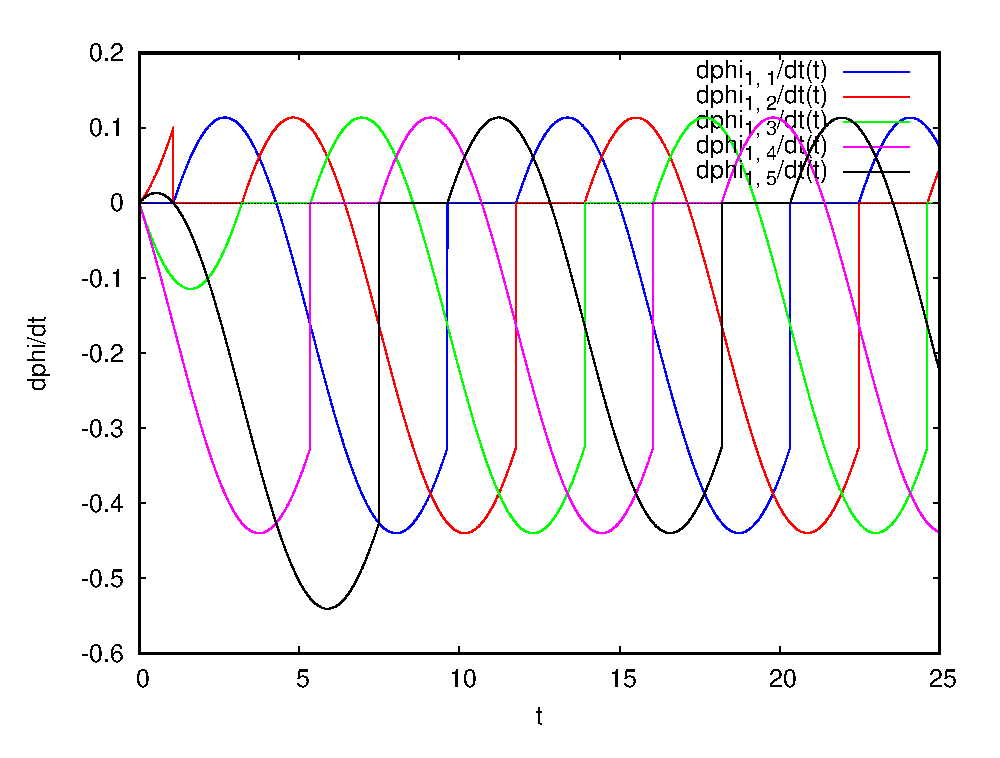
\includegraphics[scale=0.33]{pic/self_rot_25/rol_vel.eps}
        \caption{Угловые скорости роликов}
        \label{fig:self_rot_25_rol_vel}
    }
    \newline
    \subf{0.3\textwidth}{
        \centering
        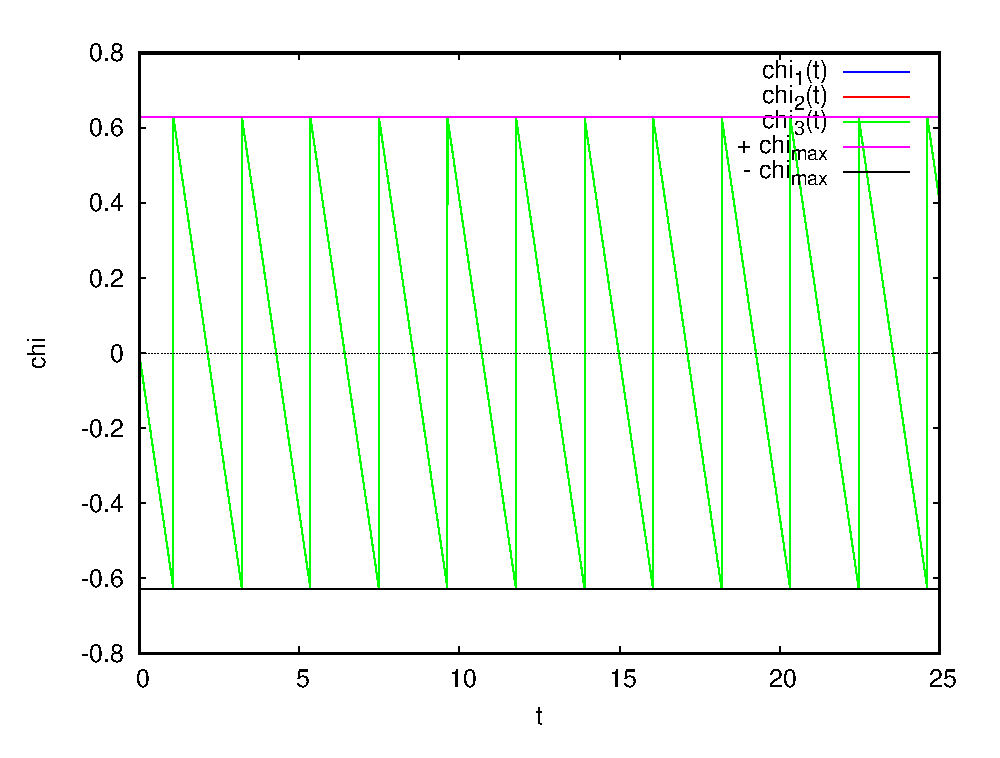
\includegraphics[scale=0.33]{pic/self_rot_25/chi.eps}
        \caption{Углы поворота колес}
        \label{fig:self_rot_25_chi}
    }
    \hspace{10pt}
    \subf{0.3\textwidth}{
        \centering
        \includegraphics[scale=0.33]{pic/self_rot_25/theta.eps}
        \caption{Угол поворота экипажа}
        \label{fig:self_rot_25_theta}
    }
    \hspace{10pt}
    \subf{0.3\textwidth}{
        \centering
        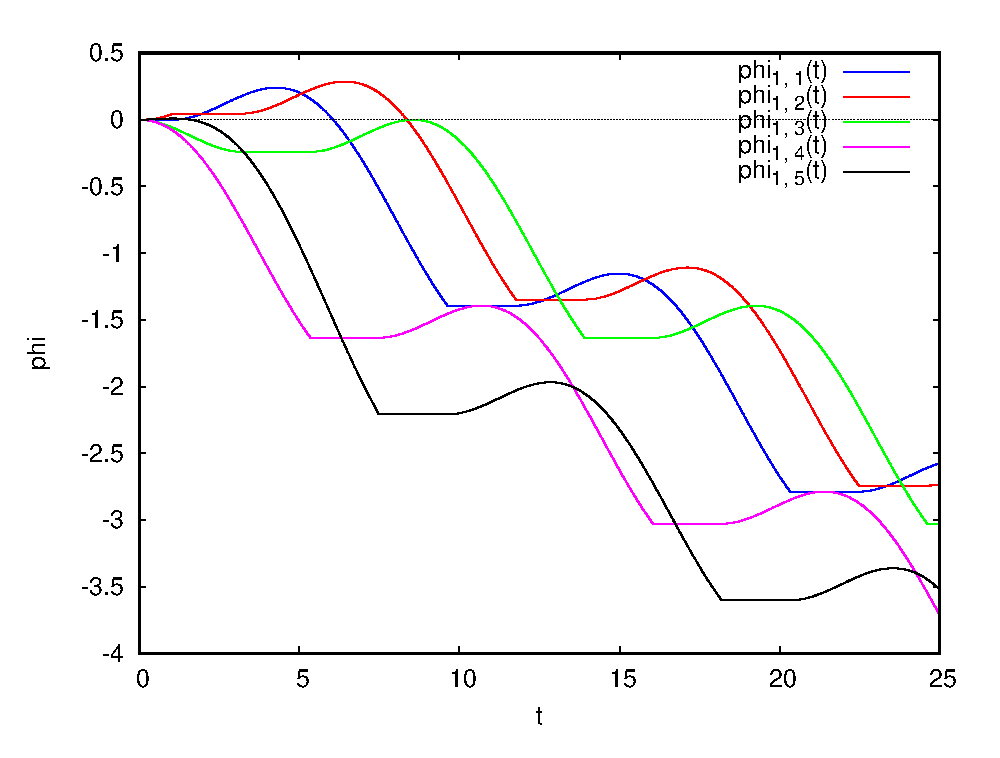
\includegraphics[scale=0.33]{pic/self_rot_25/rol_ang.eps}
        \caption{Углы поворота роликов}
        \label{fig:self_rot_25_rol_ang}
    }
    \caption{Вращение экипажа вокруг своей оси}
\end{figure}

\newpage

\subsection{По прямой}

\begin{figure}[h]
    \subf{0.3\textwidth}{
        \centering
        \includegraphics[scale=0.33]{pic/straight_100/kin_en.eps}
        \caption{Кинетическая энергия}
        \label{fig:straight_100_kin_en}
    }
    \hspace{10pt}
    \subf{0.3\textwidth}{
        \centering
        \includegraphics[scale=0.33]{pic/straight_100/v.eps}
        \caption{Скорость центра масс}
        \label{fig:straight_100_v}
    }
    \hspace{10pt}
    \subf{0.3\textwidth}{
        \centering
        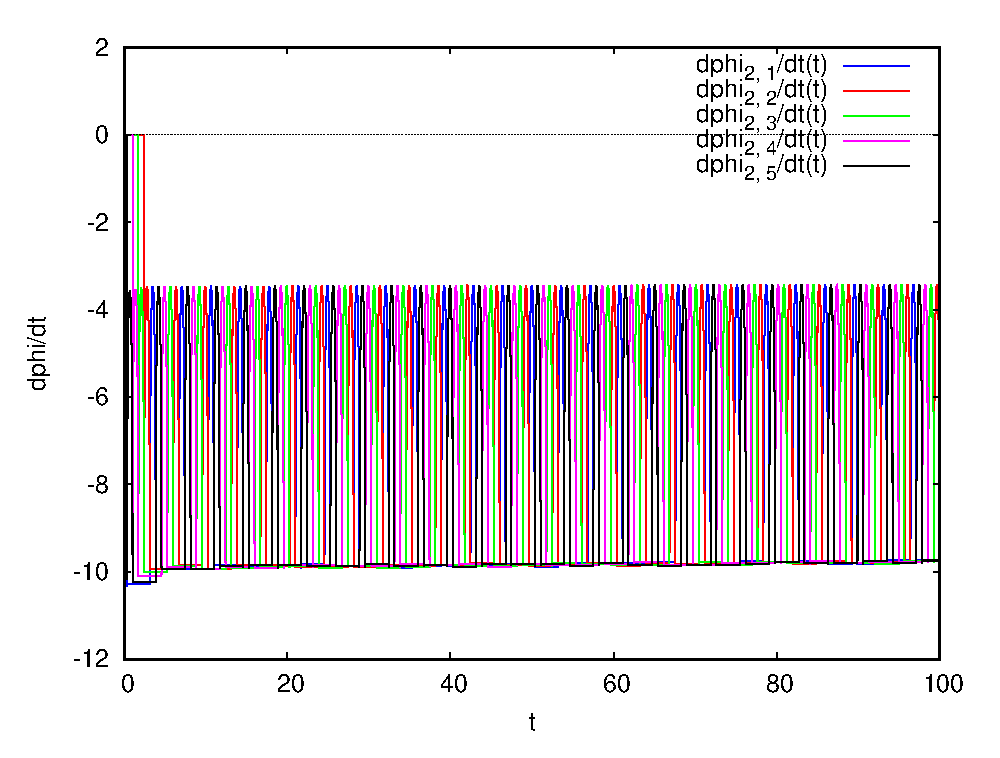
\includegraphics[scale=0.33]{pic/straight_100/nus2.eps}
        \caption{Угловые скорости роликов на заднем колесе}
        \label{fig:straight_100_nus2}
    }
    \newline
    \subf{0.3\textwidth}{
        \centering
        \includegraphics[scale=0.33]{pic/straight_100/nu3.eps}
        \caption{Угловая скорость экипажа}
        \label{fig:straight_100_nu3}
    }
    \hspace{10pt}
    \subf{0.3\textwidth}{
        \centering
        \includegraphics[scale=0.33]{pic/straight_100/traj.eps}
        \caption{Траектория}
        \label{fig:straight_100_traj}
    }
    \hspace{10pt}
    \subf{0.3\textwidth}{
        \centering
        \includegraphics[scale=0.33]{pic/straight_100/nus1.eps}
        \caption{Угловые скорости роликов на переднем колесе}
        \label{fig:straight_100_nus1}
    }
    \newline
    \subf{0.3\textwidth}{
        \centering
        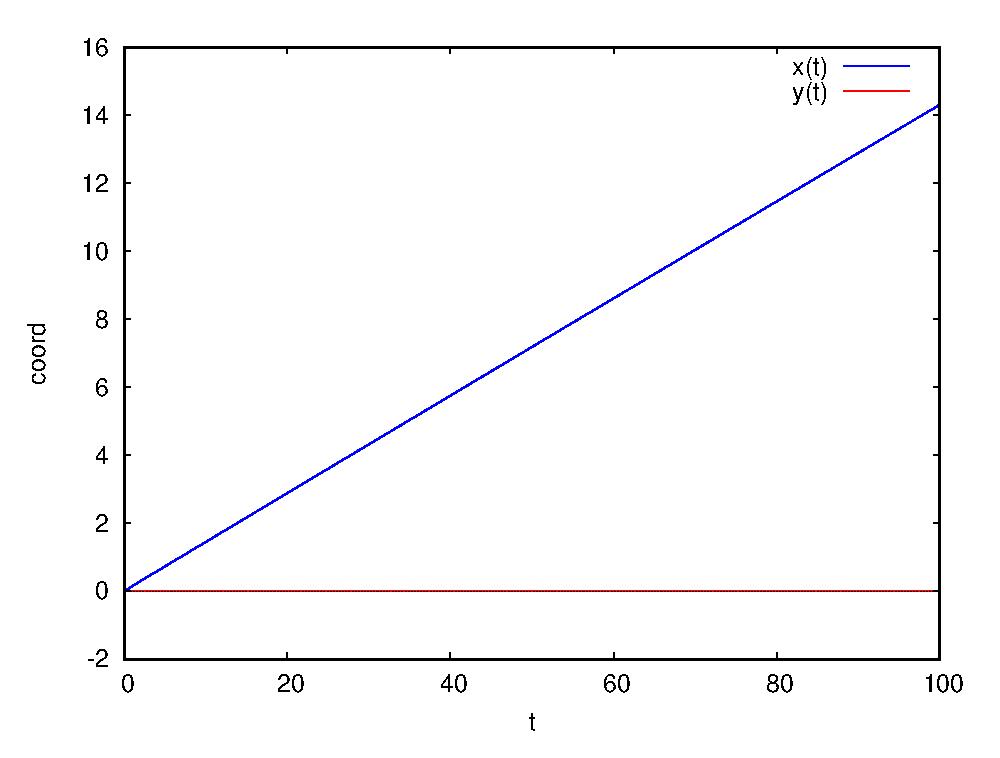
\includegraphics[scale=0.33]{pic/straight_100/xy.eps}
        \caption{Координаты центра масс}
        \label{fig:straight_100_xy}
    }
    \hspace{10pt}
    \subf{0.3\textwidth}{
        \centering
        \includegraphics[scale=0.33]{pic/straight_100/phi1.eps}
        \caption{Углы поворота роликов на переднем колесе}
        \label{fig:straight_100_phi1}
    }
    \hspace{10pt}
    \subf{0.3\textwidth}{
        \centering
        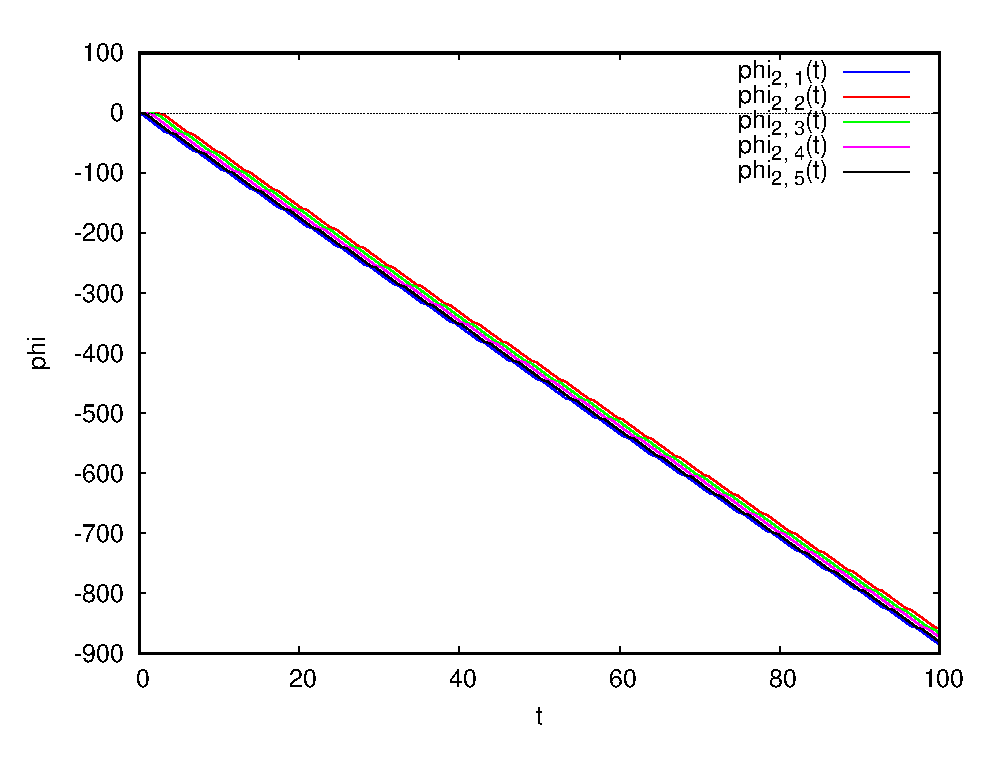
\includegraphics[scale=0.33]{pic/straight_100/phi2.eps}
        \caption{Углы поворота роликов на заднем колесе}
        \label{fig:straight_100_phi2}
    }
    \caption{Движение экипажа по прямой}
\end{figure}

\newpage

\subsection{С закруткой}

\begin{figure}[h]
    \subf{0.3\textwidth}{
        \centering
        \includegraphics[scale=0.33]{pic/wrench_1000/kin_en.eps}
        \caption{Кинетическая энергия}
        \label{fig:wrench_1000_kin_en}
    }
    \hspace{10pt}
    \subf{0.3\textwidth}{
        \centering
        \includegraphics[scale=0.33]{pic/wrench_1000/v.eps}
        \caption{Скорость центра масс}
        \label{fig:wrench_1000_v}
    }
    \hspace{10pt}
    \subf{0.3\textwidth}{
        \centering
        \includegraphics[scale=0.33]{pic/wrench_1000/nu3.eps}
        \caption{Угловая скорость экипажа}
        \label{fig:wrench_1000_nu3}
    }
    \newline
    \subf{0.45\textwidth}{
        \centering
        \includegraphics[scale=0.33]{pic/wrench_1000/traj.eps}
        \caption{Траектория центра масс}
        \label{fig:wrench_1000_traj}
    }
    \hspace{10pt}
    \subf{0.45\textwidth}{
        \centering
        \includegraphics[scale=0.33]{pic/wrench_1000/theta.eps}
        \caption{Угол поворота экипажа}
        \label{fig:wrench_1000_traj}
    }
    \newline
    \subf{0.45\textwidth}{
        \centering
        \includegraphics[scale=0.33]{pic/wrench_1000/nus1.eps}
        \caption{Угловые скорости роликов на переднем колесе}
        \label{fig:wrench_1000_nus1}
    }
    \hspace{10pt}
    \subf{0.45\textwidth}{
        \centering
        \includegraphics[scale=0.33]{pic/wrench_1000/phi1.eps}
        \caption{Углы поворота роликов на переднем колесе}
        \label{fig:wrench_1000_phi1}
    }
    \caption{Движение экипажа с закруткой}
\end{figure}
